\documentclass[11pt,a4paper]{article}
\usepackage{natbib}
\usepackage{a4wide}
\usepackage{graphicx}
\usepackage{lmodern}
\usepackage{fullpage}
\usepackage{draftwatermark}
\SetWatermarkText{DRAFT}
\SetWatermarkScale{2}

\pagestyle{plain}
\title{\textbf{Changing the delivery of primary care, and how to learn from history}}
\author{Dr Greig Russell, \\ BSc BMedSc, MBChB, BA, PGDipCEM \\ MAAFP, FRNZCGP, FRNZCUC, FACHI}
		\date{\today}
		
\bibliographystyle{apalike}

\usepackage{graphicx}
\begin{document}
\maketitle
\Large{\textbf{Report for ?}}

\Large{\textbf{Professional Practice (152.894)}}
\newline
\newline
\newline
\begin{figure}[htp]
\centering

\includegraphics[scale=0.6]{PN.png}
\caption{Palmerston North's square at night}
\label{}
\end{figure}

\pagebreak
\section{Executive summary}
Opening in rapid succession within the wider MidCentral District Health Board are large Integrated Family Health Care Centres. These centres are amalgamations of smaller 1-4 General Practitioner surgeries and provide care for ~15,000-20,000 patients. Although these have been under development for some time, enough have now been developed that most patients across the district will receive their General Practice care through an IFHC.\\

This is really the third phase of the changes that the district has undergone in the last 15 years. Health has realise the importance of primary care to deliver an affordable, accessible, and effective health service. Indeed this is one of the central tenets of the 2016 Health Care Strategy\footnote{http://www.health.govt.nz/publication/new-zealand-health-strategy-2016}.\\

This report will consider the previous two reforms, to understand, the intentions of the reforms, the impacts of the reforms and how those impacts might shape the future.\\

To achieve this the report will describe the use of new Health Informatic tools that uses techniques like Graphic Information systems, statistical process controls and time series analysis. With these analysis new insights can be developed and understood through new economic models like Game Theory.\\

The report considered the impacts of the primary health care strategy. The main finding was that General Practice had moved to being a health care retailer. General Practices now compete with other providers of goods and services for the consumer's disposable income. Practices have moved to align themselves with maximum availability for those who can afford to pay, but reducing equity of access for those who can not. Capitation funding will be found to act as a barrier for entry into the market. Without free movement, classic supply and demand correctly described problems with capacity while providers charge a premium through scarcity.\\

This may explain the impact of the Government increasing the full funding of primary care provision to all children under 13 years of age. This seemingly innocuous change in primary care funding has unleashed a substantive and unsustainable change in Emergency Department utilisation, with little impact on General Practice or apparent improvement in access. \\ 

\subsection{Recommendations}
 
\begin{enumerate}
\item That MidCentral DHB as the funder of care becomes the governance body for the delivery of both primary and secondary care.
\item That the concept of Primary Care is expanded from just General Practice to include Iwi providers, Urgent Care clinics, Pharmacists, midwives and NGO.
\item That needs of the population becomes the primary driver for care delivery decisions, with investment focusing on delivery equity of outcomes not quantity of inputs. 
\item That the DHB will need to invest in developing services to provide the outcomes needed to optimise population health for the district and provide adequate access to community based care.
\item That the DHB provides management support and advice to the newly formed IFHC, to recognise that their business survival is intimately linked to the business survival of the DHB itself.
\item That management and governance of the health sector needs to be driven by the analysis of data using modern "big data" techniques, which will require some small by DHB scale investment.
 
\end{enumerate}
\pagebreak

\tableofcontents

\pagebreak
\pagebreak

\listoffigures

\pagebreak
\section{Introduction}
Primary care delivery within the MidCentral District Health Board (MDHB) region is currently undergoing its biggest change since the introduction of capitation funding and the associated shift to population health.\\

There has been a drive to amalgamate small practices into larger Integrated Family Health Centres (IFHC), where groups of ten or more doctors, plus associated nursing staff provide primary care for 15,000-20,000 patients. \\

This is the third major reform of the local primary care health sector in the last 15 years and the second in the last two years. Both of the previous reforms were changes in national health policy, while the development of the IFHC system was a local initiative. \\

This report will seek to understand the impacts of the previous two reforms. Through developing an understanding of the impacts, both the analytic tools and the strategy needed for the ongoing management of primary health care delivery can be developed.\\ 

The previous reform was when on the 1st July 2015 the government implemented its election promise to make care free for all children aged 6-12 years who were registered with a Primary Healthcare Organisation (PHO)\footnote{http://www.health.govt.nz/your-health/services-and-support/health-care-services/visiting-doctor/zero-fee-doctors-visits-children-aged-under-13}.\\

For primary health care providers, the focus was about getting adequate compensation to offset any income loss\footnote{http://www.radionz.co.nz/news/political/271689/doctor-visit-promise-falls-short}. Within the secondary care environment, little comment was heard. This funding change was only seen as impacting primary care and even then in a marginal sense.\\

What happened was totally unexpected as this reform seemed simple, almost administrative and clearly aimed at only General Practice. Instead of more patients  attending their General Practitioners, patients flooded both the local community based urgent care clinics and the hospital Emergency Department.  The local urgent and emergency care systems were an remain overwhelmed. The record numbers attending acute services have now become the new normal, but this is placing pressure on unchanging hospital budgets. \\

This unexpected result to a "minor" funding change was contrary to what was expected under the Primary Health Care strategy when it was released by the then Minister of Health, Annette King \citep{king2001primary}. As envisaged, the "free under 12 years" funding shift should have lead to better access to primary care and a focus on population based proactive preventative care. The intention of the 2001 reforms was to move away from reactive, fee for service care delivered by only doctors. Instead it would be multidisciplinary team based care focusing on the health of the entire population and focusing on wellness \citep{king2001primary}. The envisaged system should have not just coped, but rather had its mandate extended by reducing financial barriers to attendance. The need then is to understand the impacts of the primary health care strategy on primary health care delivery so as to be able to understand the paradoxical effects of extending the scheme in 2015.\\

With the election of the fifth Labour government in 1999, Minister King had inherited a health system that had been through a series of changes, but which had remained the same from a patient perspective for many decades. Until the early 1990s, the New Zealand primary care system had been one of a state subsidy based on a fee for service by a doctor \citep{gauld2006new}. With the neo-conservative health reforms of the early 1990s the split between funders and the providers of care was introduced, along with increased competition between providers as part of a drive for achieving the economic efficiency inherent within the true free market. General Practitioners were allowed to form Independent Practitioner Associations (IPAs) so as to form groups of sufficient size, so that primary care providers could participate effectively in a competitive health care model. These IPAs continued to be predominantly GP led and, as organisations, they remained focused on protecting their General Practitioner members from any negative impacts of the neoliberal health reforms \citep{malcolm1999new}. Some IPAs achieved successes through profit sharing arrangements with the new funding bodies, but essentially from a patient perspective it was business as it had always been. The Government funding of primary care provided less than 10\% of income during practice in this era. This percentage of practice income provided by the state to subsidise patient fees and ease access to community based health care was reduced each year. As the rate of inflation was greater than the rate by which the subsidy increased, the subsidy became an increasingly smaller component of practice income. Even this limited subsidy applied only if the doctor saw the patient and did not apply if the patient saw the practice nurse. This activity based funding system led to absurdities through valueless over servicing. \\    

The Primary Health Care Strategy wanted to achieve a more fundamental reform of primary care and had broader aims \citep{king2001primary}. Under the strategy, health care was to be about the health of entire populations and focused on providing preventive health care delivered by multidisciplinary teams. The funding of primary care was to be on a capitation basis where subsidies to practices were on a fixed income per annum per enrolled patient and not on an activity basis. It was in a practice's financial interest to spread consultations across all team members as this improved profitability by increasing the number of patients the practice could enrol. Only by focusing on preventive health care could the required reduction in consultation rate per patient be achieved for the practice to live within its means. \\

The shift to capitation-based funding also removed the funding barrier to non-medical providers participating in health care provision. Indeed, a fixed income should have encouraged practices to use cheaper nurses to provide patient care than more expensive doctors whenever possible. Indeed, it was imagined that nurses could open their own practices without doctors. Envisaged in the strategy, was that all professional groups could now contribute to overall community health outcomes, with each team member working at the top of his or her scope of practice. \\

Driving the adoption and success of the new strategy was an increase in overall health funding of \$500 million per year from 2002-2008 \citep{gauld2006new}. Increased demand for health care, especially in areas of deprivation, was to have been driven by this dramatic increase in funding \citep{king2001primary}. From the perspective of "supply and demand" microeconomic theory, the Primary Health Care Strategy aimed to establish a local free marketplace, with funding to enable all patients to participate as they sought the best deal from multiple suppliers or practices. Patient demand was to drive primary health care to the optimal allocative efficiency of resources to meet their health care needs. It was envisaged, moreover, that the behaviour of the primary health care market in a given locality would be regulated automatically by the 'invisible hand' or inherently self-regulating nature of a free market. In this situation, the focus of the Government was to be on ensuring participation of those from areas of deprivation and poverty. \\ 

The challenge in this field of study, has been how to evaluate the actual impacts of the strategy on society and the health system. As without an understanding of how the strategy impact utilisation of primary care, there will not be an understanding of how increasing funding for one group to receive easier access to community case lead to a dramatic rise in utilisation of the emergency department.

\pagebreak
\section{Literature review}
Studies considering the impacts of the Primary Health Care Strategy have produced conflicting responses to date. \citet{hefford2005reducing}, examined the strategy's results 15 months after implementation. The authors described the development of performance indicators to allow any effects of the strategy's introduction to be tracked, especially with regards to correcting inequities. The study described  how this increased funding was cumulatively supplemented for those living in areas of high social deprivation by an additional 20\% per enrolled patient in a practice, and by another 20\% for every self-identified Maori or Pacific Islander, who enrolled (p. 14) in the practice \citep{hefford2005reducing}. One clear intention of the strategy was to shift these groups of patients from being financially undesirable to being financially highly desirable. This shift would attract providers to areas of high need and hence correct long-standing health inequities to exploit this new opportunity. If the total enrolled population of ethnic minorities and those who lived in areas of high social deprivation was above 50\% of the locality's enrolled population then further funds were provided to every practice in the locality. \citet{hefford2005reducing}, found that those most in need had enrolled in greater numbers than the general population. The overall level of funding that these ethnic minorities and those patients from socially deprived areas  received was 25-60\% higher under the strategy than under the previous funding formula. The authors argued that this reduction in cost for these previously undesirable patients, and their observed greater uptake will lead to improved health outcomes. The authors described overseas studies which found this exact effect.\\

\citet{howell2005restructuring}, was less optimistic than Hefford. She argued that the strategy is the adoption of an insurance model where the individual practice in effect becomes an insurance agency, where the capitation is a premium that pays for a fixed quota of care. For Howell, once the quota of care is exceeded by the patient, the risk of the financial cost of ill health is transferred to the practice. She identified two groups of patients who will use excess care as compared their capitated funding and so create financial risk for the practice. The practice will then (probably) mitigate that chance by passing the costs of excess use back to the patient through fee rises to all patients.\\

Her first group was the worried well, who may seek more care than their capitation funding allowance, attracted by the reduction in prices. The second group who might care above their capitation funding was those patients with a chronic illness, especially those with multiple comorbidities, attracted by lower prices to get necessary care. The amount of care sought again is in excess of the capitated allowance.\\  

To manage these financial risks the patients fees would rise, especially within a small cohort of patients, such as the 1-3 doctor practice. As spreading the risk of the few across a large cohort of patients would powerfully mitigate these potential risks, Howell argued that any fee rises have adverse effects on the effectiveness of the Primary Health Care Strategy. The affluent, given their greater weekly income, would experience against a background of higher disposable income as only a relatively small reduction in fees affordability. Any fee rise would have a disproportionate effect for poorer people, though, given their initial lower weekly income, so once again fees would act as a barrier to those seeking appropriate care. These increasing costs would act as a disincentive particularly for the preventative care of those with chronic illness and need more frequent attendances to achieve maximal outcomes.  \citet{howell2005restructuring} described how, in order to prevent fees rising, the then Labour government would have had to restrict the historical right for General Practice to control their charges independent of external regulation and change the historical fundamental business model of General Practice away from individual ownership to a collective.  The Labour government was unable to achieve either change.  \\

For \citet{howell2005restructuring}, then, after an initial period of readjustment the patient costs would rise, and the focus of General Practice would remain on those who can afford to be sick. Howell argued for the adoption of an actual insurance model. If such a model was adopted, then the financial risk of chronic illness and the ability to manage locality derived utilisation patterns would be carried by a much larger group of patients and providers than was achieved under the Primary Health Care Strategy by 2005. This would reduce the drivers towards fee increases and its associated distortions to the system.\\

Depressingly, more recent evidence seems to support Howell's pessimism rather than Hefford's optimism when considering the potential of the strategy to achieve its goals of reducing health inequity within the population by providing equality of access. \citet{jatrana2009primary}, described the impact of the strategy on primary care utilisation. Those with the greatest number of current comorbidities, current smokers, those who felt their health was poor, those who had limited education and those who came from the most significant levels of social deprivation - were all likely to delay seeking medical review and were much more liable to delay filling a prescription.  As an example, consumers who were in the NZ Index of Deprivation of 5 or higher were 18.01 times more likely to delay seeking medical review as compared to the lowest group in the NZDep and 24.47 times more likely to delay filling any prescription. \citet{cumming2008reforming}, considered  that although the Labour government was injecting considerable extra funding each year under the strategy, this increase of financing was not passed on as fee reductions.  In fact, by 2005, patient charges, rose on average for adults by 18\% (or \$4.30 / consultation). In practices with the higher levels of social deprivation and large concentrations of ethnically disadvantaged patients, the fees dropped by 20\% (or \$4.40 / consultation) for adults. This reduction represented a small percentage drop in overall household weekly income, militating against its effectiveness in reducing health equity.  The authors described how the most significant impact of the rise in health funding during the implementation of the strategy was the 58\% increase in GP income from \$97,220 to \$153,886. This growth in practitioner income together with overall patient fee rises supports Howell's opinion that the GPs continued to manage income from fees as they had done previously, without adopting a managed risk approach, and that they continued to use fees to manage fiscal risk from chronic illness. \\

\citet{howell2005restructuring} prediction was that fees would again become the primary economic driver for the financial stability of practices. Driven by the ageing  population, there would an associated projected rise in the number of patients with chronic illnesses and multiple comorbidities that would lead to an increased  average utilisation rate greater than that provided under the capitation funding rates. The increased government funding provided through the initial roll out of the Primary Health Care Strategy would have offset the impact of increased utilisation on practice income. After the annual growth in funding ceased then the percentage of income from capitation would have to fall as a percentage of total practice revenue, and a rise in the fees derived income would be needed to offset that reduction in the face of rising utilisation.\\

New methodologies for studying such problems have become locally available with the arrival of new (or at least new within the DHB) analysis programs and statistical analysis methods. Although first developed at Auckland University\footnote{https://en.wikipedia.org/wiki/R\_(programming\_language)}, R statistical language has evolved to becoming accessible to non-expert statisticians. \citet{khoury2014big}  describe the hope that with advanced data analytic techniques,  novel predictive hypotheses can be generated from new large data sets so opening up new approaches to patient care. Data is transformed through the use of high level data analysis applications like SAS or R and through the use of techniques like statistical modelling, data mining or machine learning. These tools can manage both the scale and complexity of very large data sets, so allowing the development of the hoped for novel clinical or organisational insights \citep{reshef2011detecting}.  More recently the potential to be found in data analysis within health care, has also been embraced in the newly released revamp of "New Zealand Health Care Strategy" \footnote{http://www.health.govt.nz/publication/new-zealand-health-strategy-2016}. In the strategy, data analysis is one of  the five key tenets needed for the development of a sustainable health system. \\

This report will use analysis techniques like statistical process control to understand the operational flows within the emergency department \citep{rosemann2015six, cheng2015run, epprecht2015statistical}. Statistical process control technqiues have already been used to study the operational function of emergency departments \citep{pimentel2015statistical} and are widely used within the field of quality improvement \citep{provost2011health}.\\

Previous studies on the utilisation of the Emergency Department had noted a marked geographical maldistribution. This result was unexpected, except by the Emergency Department staff who had known it all along. They assumed everyone else also knew, so they were surprised that everyone else did not know. To consider the impact of geography on the health system and consumer behaviour, Geospatial Information System (GIS) and Games Theory analysis techniques were used.\\

In economics, Game Theory is used to explain or develop a winning economic strategy. All businesses that adopt this optimal strategy flourish or at least survive while those that do not inevitably perish. A strategy can focus on the range of goods or access to the market. In health markets like primary care provision, then the range of products and internal business model is similar to all providers, so the  only variable that can change is the market's ability to access that provider \citep{dinar2008game}. \\

To demonstrate this concept, the most frequently used example describes two ice cream vendors on a beach. The first sets up in the middle of the beach and gets unique access to 100\% of the market. With the arrival of the second, the profit-maximising position for them both on the beach is for one to be at 25\% along the beach and the other at 75\%. The reality is both will be found in the middle, with both ice creams vendors beside one another selling the same goods at the same price. Game theory predicts this because if one vendor suddenly moves to the middle of the beach, then they will control 75\% of the market, a considerable gain. The other vendor, who stayed still, will only control the other 25\% position. The profit maximising position may therefore create the most profit, but also promotes the most risk. If both move to the middle, neither can lose a share of the market to the other and so this is the position where neither can lose from the actions of any one else, and no party consistently gains by moving away from it. The middle position, which minimises the risks to all players, or the position of no regrets is called the Nash Equilibrium. In a stable, mature market, the geographic position of business clusters is described as  the Nash Equilibrium between the economic forces under which the businesses operate. If two groups of businesses have similar Nash equilibrium positions as seen from geographic locations, then they operate under similar economic forces. If they are in different locations then the two sectors are reacting to various economic drivers. \\

Game theory has been applied to the development of health systems. \citep{dobson2004sustainable}, used the combination of game theory and social network analysis to understand the development of an integrated local mental health initiative. This study found that the outcome of the initiative for participants was driven by the social network in which decisions were made. The analysis was made by analogy to the famous game called the "Prisoner's dilemma", where the players get a moderate adverse outcome through cooperation, while one would receive a favourable outcome and the other a much worse through not cooperating. This study suggested that, by failing to consider how to optimise their position, the participants left themselves vulnerable to the worst case outcome. \\

\citet{tarrant2010continuity}, have used Game Theory to understand the drivers behind patient trust of primary care physicians and how that changes with time. There were difficulties previously in understanding engagement, whether long term relationships lead to the evolution of trust in primary care physicians and if so, the reason behind this development. The authors' use of Game Theory enabled them to describe the underlying "game" of the therapeutic relationship. They found that patients started from a position of the generic physician encounter based on a social construct of the generic physician consultation. Game theory predicts that by repeated individual encounters, mutual benefit from the relationship develops as both seek insurance against "the shadow of the future" \citep{tarrant2010continuity}. Each participant makes no assumption of each others motivation. Indeed ill health is the shadow for the patient while financial insecurity or clinical medico-legal risk  are drivers for the physician. Game theory predicts that even without any shared motivations the optimal position for both is the development of a long term relationship to address clinical problems.  This study is not testing Game Theory but is using Game Theory to understand a social phenomenon. \\

\citet{chapman2012using}, used Game Theory to investigate incentives for uptake of annual influenza vaccinations.  The study found that when the incentives reflected self-interest the older group of players got vaccinated while the younger group did not. When the incentives were changed to reflect outcome for the total community (a "get vaccinated to protect your grandmother" style approach) the new Nash equilibrium position reflected a group-optimal utilitarian position. This study again used Game Theory to understand clinical behaviour in the community. It also showed the use of Nash equilibrium to illustrate changes in the net position of a population of non-cooperating individuals. \\

Game theory is in one respect an emergent economic theory, yet it is also an established theory, with an increasing repertoire of useful applications in different situations. \\

\pagebreak
\section{Method}
Palmerston North is effectively a geographically isolated city in the mid central of the North Island, at least as far as access to medical care. It is the regional hospital for the provision of cancer treatment services, and usually nearby provincial areas refer to Palmerston North Hospital. The nearest tertiary hospital is approximately two hours drive away, which when considering illness and health care is an impractical distance.\\

\begin{figure}[htp]
\centering
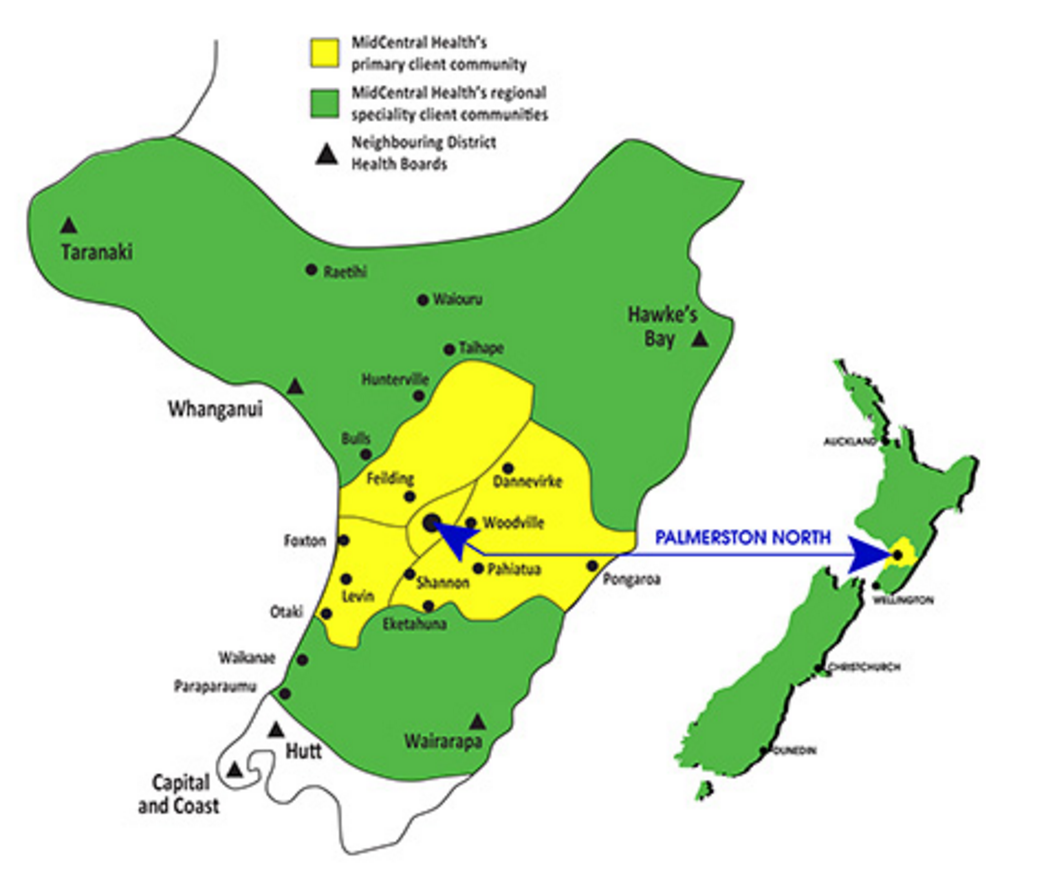
\includegraphics[scale=0.5]{fig1.jpg}
\caption{The location in New Zealand and the total area of responsibility for MidCentral DHB}
\label{MidCentral District Health Board}
\end{figure}

Conveniently Palmerston North is laid out as a rectangle, with deprivation believed to lie in equally distinct quadrants, although this was not later confirmed.\\

\begin{figure}[htp]
\centering

\includegraphics[scale=0.20]{fig2.png}
\caption{The traditional view of the economic layout of Palmerston North. The poorest sector is the top left quadrant, the richest in the bottom right. In between lie the middle classes.}
\label{Traditional view of the spatial economics of Palmerston North City}
\end{figure}

The introduction of the primary care strategy led to the disestablishment of the previous General Practice governance structures. This in turn resulted in the loss of all data prior to the disestablishment and this was an unforeseen complication in this study. On review of the options for historical information, the assumption was made that commercial organisations, including medical practices, generate business by advertising. As part of advertising, the address is also supplied along with the nature of the business. Telephone directories are public information, and are held in the local public library. These served as the basis for the geographic data set used in this study.\\

The data collected was simply a table of names of practitioners, the address they gave in the telephone directory of the year and the nature of their practice (solo vs. small group practice vs. large group practice with over five practitioners at a single location,  General practice vs. Urgent care vs. Specialist Care). Only the  medical practices listed in the specialist medical practitioner section of the telephone directory were included. The current government is encouraging the formation of large integrated family health centres. As a byproduct of this further development, the intended location and nature of practices is also known in 2016.\\

Difficulties with using the telephone directory as a data source were immediately apparent, including, for example, occurrences such as a failure to update addresses when practitioners moved to new premises. It was, in addition,  impossible to determine whether there were omissions from the directory. Some group practices only list their medical director, not all medical and nursing staff employed there. As a consequence, the contribution of such practices to the overall provision of health care will be under estimated.  After discussion, it was decided to proceed with the limitations in the data set as no better data set was available.  \\

Clearly there are many interdependent factors in any given market that will impact on economic activity by retailers, independent of macroeconomic policy for niche markets like health. A classic example is the 2009 global financial crisis that affected all business including health. To control for these local or global effects on the whole local market, retail alcohol was chosen.  This group was selected as they provide services of similar cost, with similar hours of operation but are not subsidised by central government. Only those hotels, retail alcohol outlets and bars in the relevant sections of business section or "Yellow pages" were considered to be part of this control group. There were similar limitations in the data with regards to this group as there were for medical practitioners.\\

The analysis method comprised of two phases. The first was to use GIS to plot the changes in the geographic distribution of General Practices in Palmerston North city from 2002 - 2016. The second phase was to try to understand the distribution and changes over time against controls or alternative possible hypotheses. \\

Analysis was carried out using two tools. The network analysis and Heat maps were completed using Google Fusion tables, while the statistical analysis and visualisation of the results were completed using Google Sheets. The Graphic Information System analysis was completed using Google maps. All data was held in a secure data repository that is compliant with FISMA, ISO 27001, ISAE 16/3402 and HIPAA international standards for health data storage. In dealing mathematically  with the inherent issues in this data set, it was treated as a sample not a population. This adjustment partially compensated for the data quality issues. Classical microeconomic theory and game theory was used to consider the results of the GIS study from an economic perspective. \\

Local ethical approval for this study was obtained via the MidCentral Health Clinical Board. The Clinical Board is responsible for all local Health research undertaken within the District Health Board, including primary care.  Regional approval from the Central Health \& Disability Ethics Committee (HDEC) was not required as this study was deemed to be  a low or minimal risk. \\

\section{2001 primary care reforms}
For Game theory to have any applicability in a GIS based study there has to be geographical movement of practice location. Locally individual practices are, however,  noted for their longevity of location. This study revealed that General Practitioner turnover was greater than perceived in Palmerston North, despite the prevailing perception being focused on difficulties of attraction not retention. \\

\begin{figure}[htp]
\centering
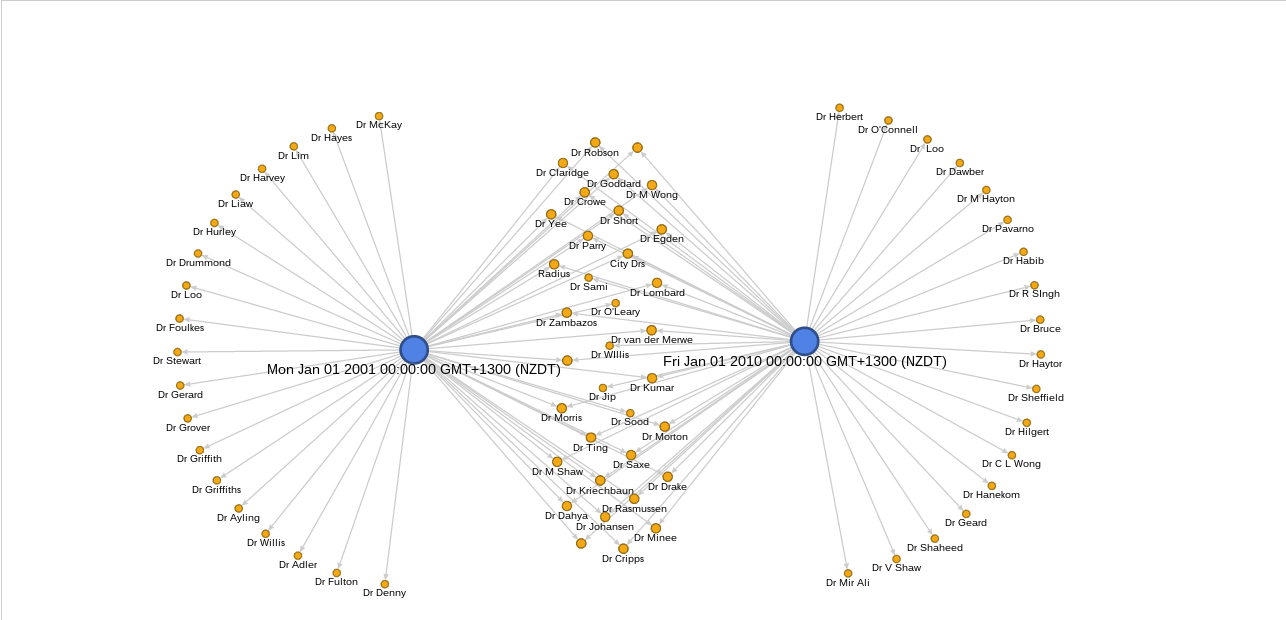
\includegraphics[scale=0.4]{fig3.png}
\caption{Network analysis showing General Practitioners present in 2002 and 2010, with the group in the middle present at both}
\label{General Practitioners present in 2002 and 2010}
\end{figure}

This turnover of practitioners was the mechanism of practitioner migration within Palmerston North. Where practitioners start new surgeries, they open them at new locations as compared to the surgeries that they replaced. The underlying basis for that decision is not conscious but does appear reactive to economic opportunities. This makes sense given the desire of any new business to be financially successful and the fact that new General Practitioners would not have any emotional or social attachment to the previous practice location.

The raw results of the telephone directories and projections for 2016 revealed a far from stable population of practitioners: there is a diminishing population of providers in Palmerston North. There is a core group of practitioners who are pivotal to the stability of supply through their longevity in their practices with a wider group of assistants or transient practices supplementing primary health care delivery. That this group is starting to approach retirement is one of the drivers to establish integrated family health centres, so as to provide a vehicle for succession planning. This reduction in the number of practices is in contrast to the ambitions of the Primary Health Care strategy, one of the aims of which was to increase access through practitioner diversity.  \\

As practitioners move into private practice, they are attracted to a specific practice configuration and this does not change this throughout their careers. To consider geographic movements of General Practice over time, a series of heat maps was developed from the 2001, and 2016 data respectively.(see figures 6 \& 7).\\ 

\begin{figure}[htp]
\centering
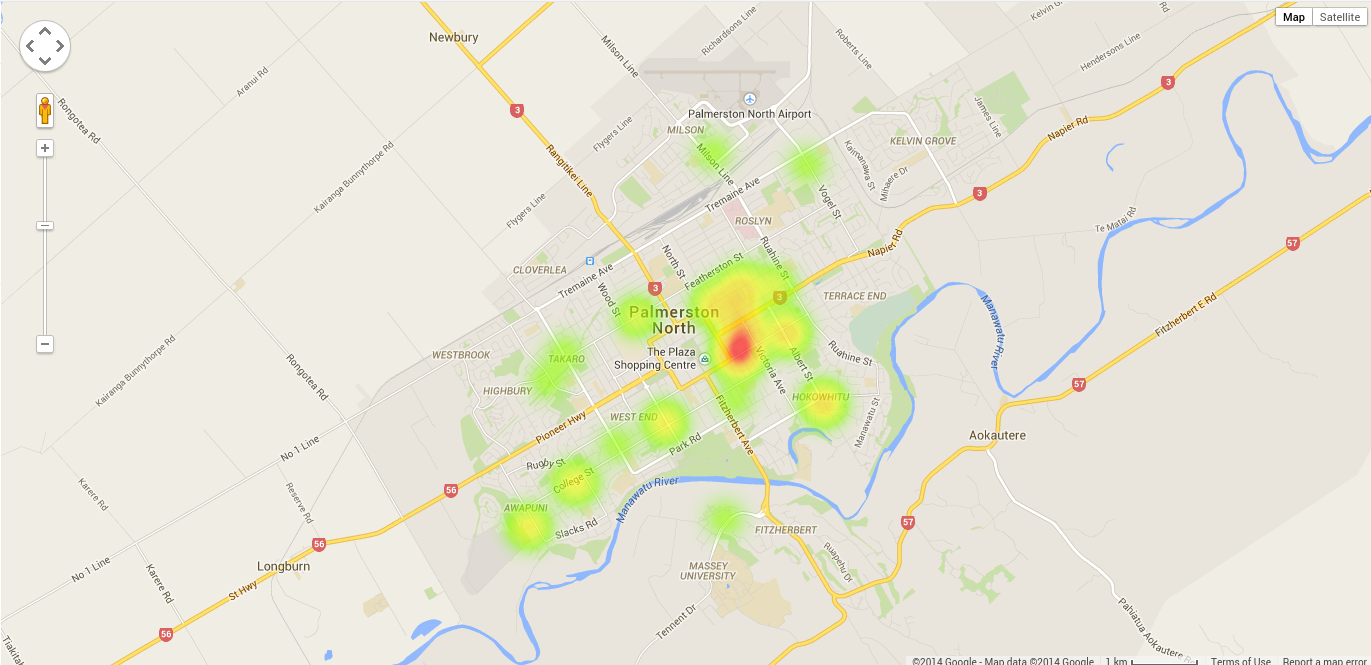
\includegraphics[scale=0.3]{fig6.png}
\caption{Heat map of the distribution of primary care provision within Palmerston North 2001. Please note that prior to the 2001 Primary Care Health Strategy there was even GP coverage of Palmerston North.}
\label{Heat map of practitioners 2001}
\end{figure}  

\begin{figure}[htp]
\centering
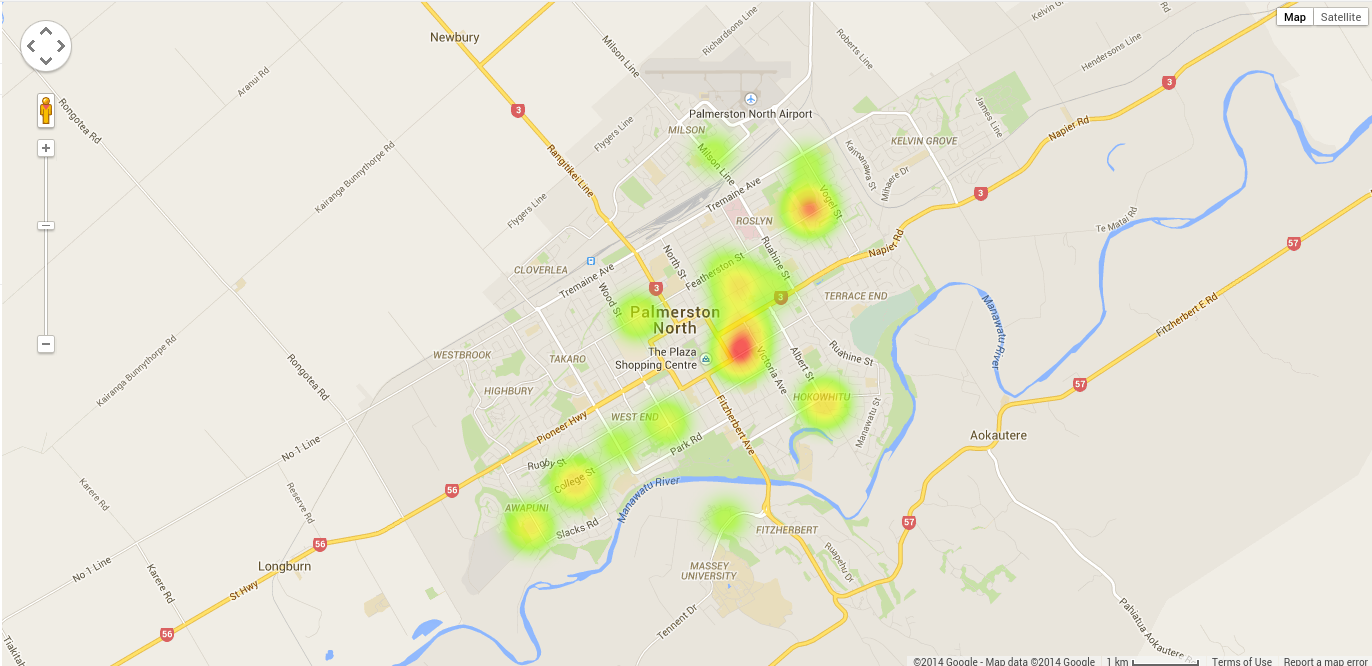
\includegraphics[scale=0.30]{fig7.png}
\caption{Heat map of the projected distribution of primary care provision within Palmerston North 2016}
\label{Heat map of the projected distribution of primary care provision within Palmerston North 2016}
\end{figure}

The distribution of primary care does not appear to match unmet clinical needs.  Consider the map of a sample of patients who presented to ED in 2015 without a current General Practitioner (see figure 8).\\

\begin{figure}[htp]
\centering
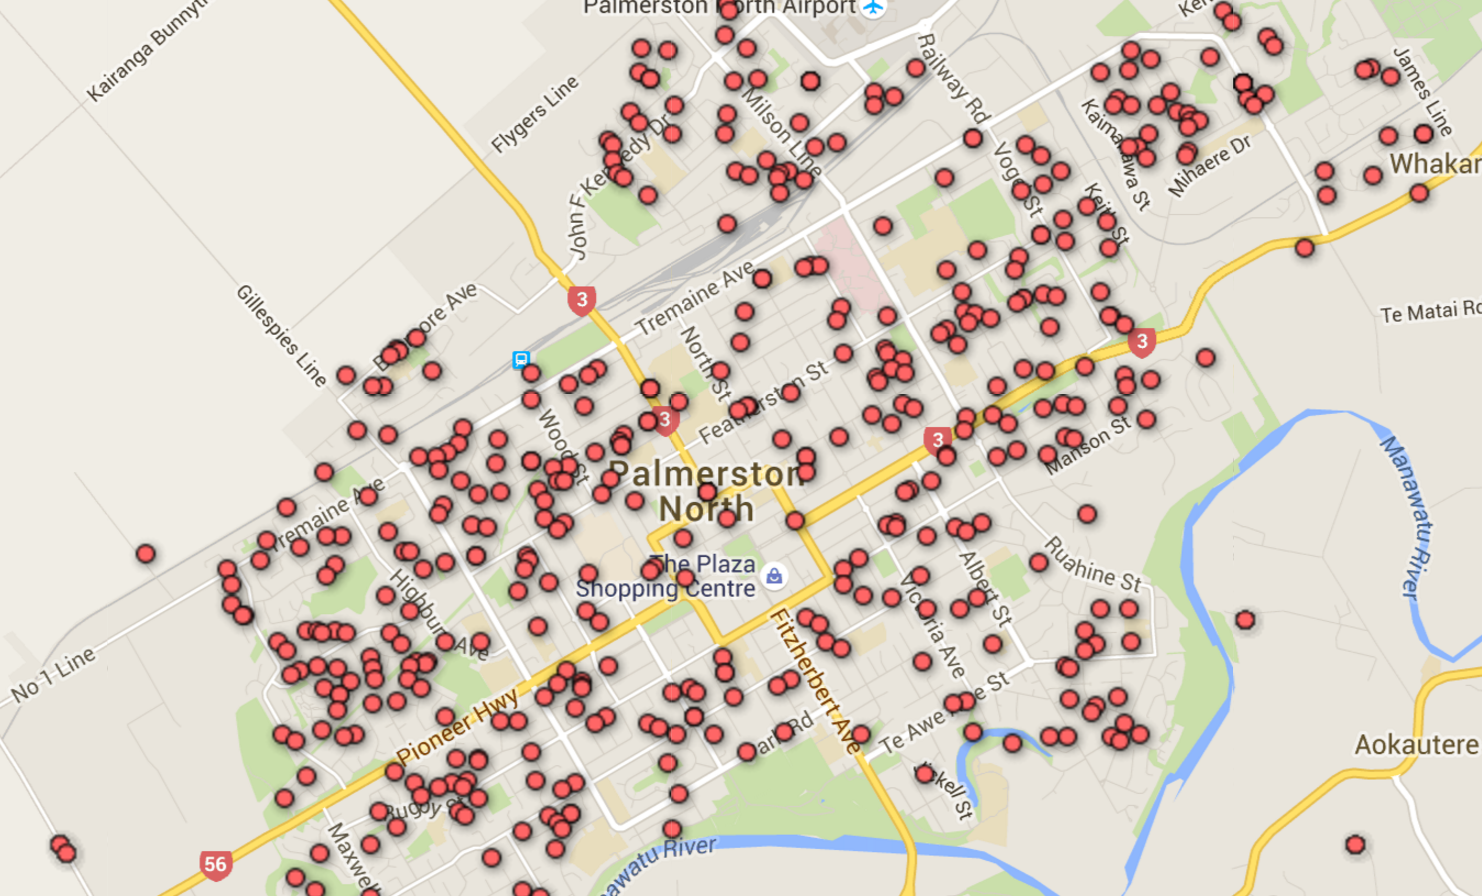
\includegraphics[scale=0.30]{fig8.png}
\caption{A sample of 1000 patients who attended Palmerston North Emergency Department,and did not have a GP in 2014}
\label{Distribution of patients with a General Practitioner}
\end{figure}

This distribution of General Practice providers is also quite different from services which aim to achieve equality of access across the town, such as the local bus service (see figure 9). There are, moreover no town planning barriers to the opening of new practices in the suburbs. \footnote{Palmerston North District Plan, R 10.8.1.4}  \\

\begin{figure}[htp]
\centering

\includegraphics[scale=0.3]{fig9.png}
\caption{Distribution of bus routes designed to maximise social equity and access by the public}
\label{Bus routes designed to maximise equity of access}
\end{figure}

\begin{figure}[htp]
\centering
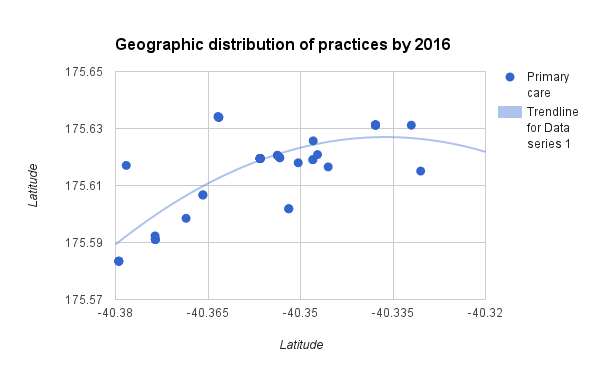
\includegraphics[scale=0.6]{Nash_GP_2016.png}
\caption{Scatterplot of General Practitioner location 2016, with a clear trend line present}
\label{Scatter plot of General Practitioner locations}
\end{figure}

Yet there is a clear pattern present underlying the distribution of General Practitioner by 2016 (see figure 10). Interestingly a similar pattern is seen when alcohol retail outlets are superimposed (see figure 11). \\

\begin{figure}[htp]
\centering
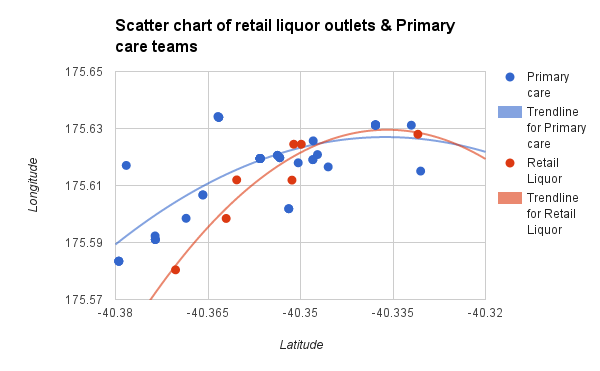
\includegraphics[scale=0.6]{Nash_GP_retail.png}
\caption{ Scattergram of both retail alcohol outlets and Primary Care providers in Palmerston North 2016}
\label{Geographic distribution of practices by 2016, with retail outlets overlaid}
\end{figure}

The distribution of both primary care and retail outlets appears to be maximised in the space between the two areas of affluence within Palmerston North (see figure 12).\\

\begin{figure}[htp]
\centering
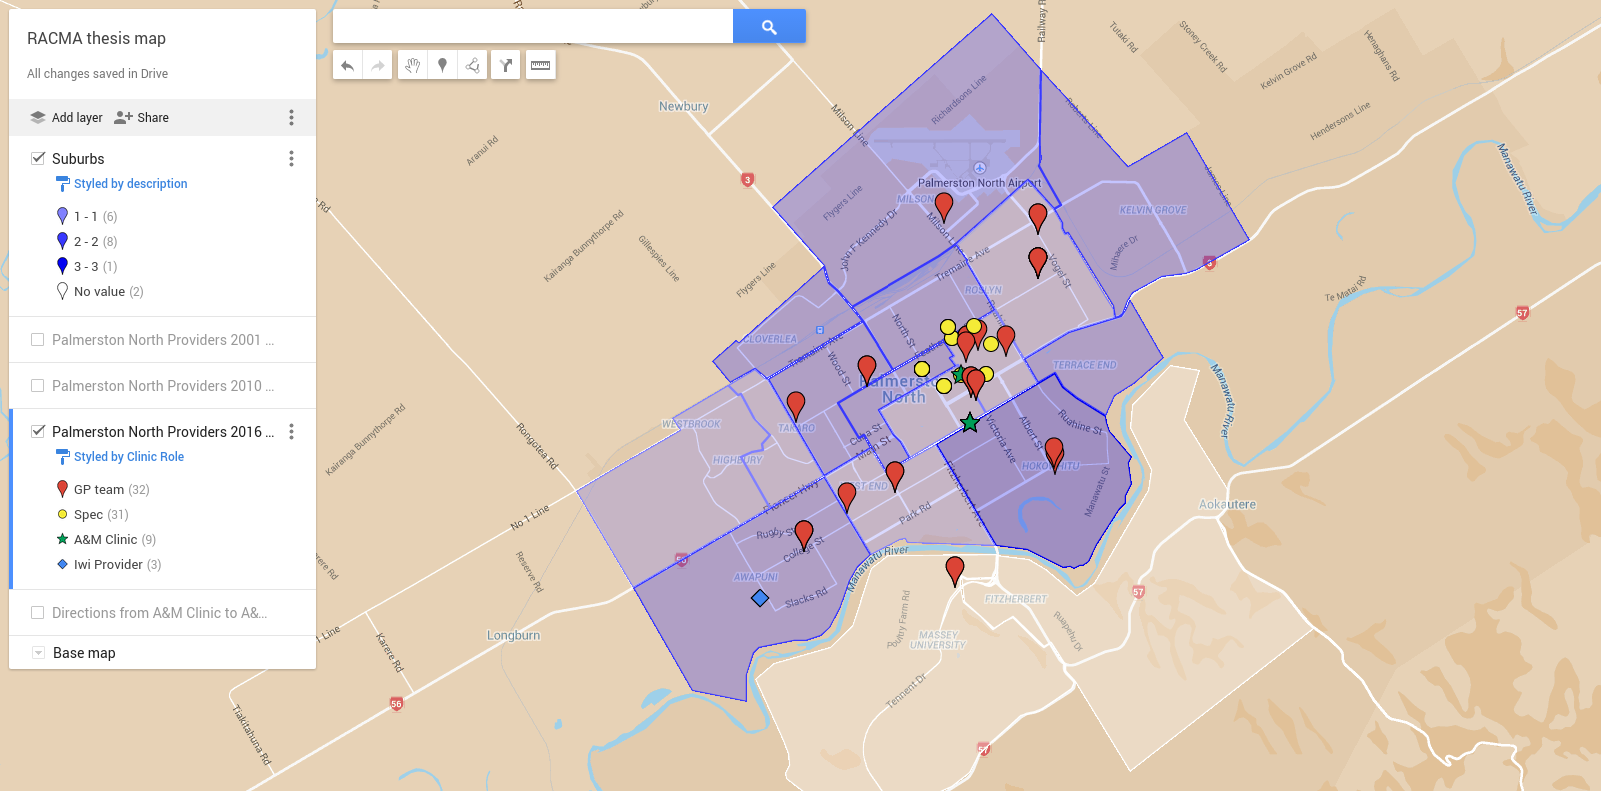
\includegraphics[scale=0.40]{fig12.png}
\caption{The distribution of both primary care and retail outlets appears to be maximised in the space between the two areas of affluence within Palmerston North.}
\label{Distribution of General Practitioners overlaid on suburb's social deprivation}
\end{figure}

In summary, the use of Game Theory to analyse the results of GIS data enables an understanding of the microeconomic forces consequent to the changes in the macroeconomic policy. In this instance, Game theory analysis supports a proof by abduction that;

\begin{enumerate}
\item The location of primary care and retail outlets in Palmerston North are on almost identical geographical arcs.
\item The location of these arcs is equi-distant between areas of maximal disposable income.
\item Game Theory predicts this equivalence if both are driven by equivalent economic drivers.
\item The distribution of providers is not associated with unmet community need.
\item The distribution of primary care providers is different from services aimed to provide equity of access.
\item There are no local barriers to practices opening in alternative locations.
\end{enumerate}

Hence, in this location primary care provision is a retail activity, not one driven by the need to achieve patient equity or to address unmet patient need. This conclusion is clearly at odds with the objectives of the Primary Health Care strategy.

\pagebreak
\section{2015 funding reforms}
Following on from the above argument, by 2015 General Practice moving to an activity driven funding model to adopting a retail service delivery model under the guise of the capitation funding model seemed to have no significant adverse effects.\\

The general practices were/are independent businesses, usually owner operated and service provision is via a series of contracts, only one of which is for the provision of primary medical care in the community with Ministry of Health. The nature of the contracts allowed the practices to effectively ignore the PHO if they wished. The funding is transferred from Ministry of Health to individual practices via the DHB and local PHO\footnote{http://www.health.govt.nz/our-work/primary-health-care/primary-health-care-services-funding-and-contracting}. The contracts themselves are national contracts between the NZMA and the Ministry of Health\footnote{http://www.nzdoctor.co.nz/news/2016/may-2016/16/increase-of-1-per-cent--in-capitation-proposed-for-general-practice.aspx}.\\

The governance of General Practice across the district was with the Central PHO.Central PHO adopted a governance model more "laissez-faire" than "accreditation" \citep{greenwood2007european}. To be fair there was considerable pragmatism to this approach. Many of the group practices are more in the nature of cohabiting solo practices sharing administrative and overhead costs. So there was no coherence for the PHO to engage with. The reality that the Central PHO was established years after many of the general practices. That the PHO went through at least four phases in its management and hence governance of the general practices further undermined the PHO's ability to adopt another style of governance. There has been no sense of the PHO being able or even being willing to provide other than a "laissez-faire" approach to governance. In fairness without obvious negative consequences beyond professional frustration in senior management, who wished to do more\\

Having won the 2014 election, the National Government proceeded to enact its manifesto promise of making the primary care for children aged six to 12 years free at point of care. This extends the age groups full funded to being birth to age 12. Funding and care arrangements for everyone 13 years and older remained the same. The scheme was listed as voluntary and opt-in, 100\% of local providers were participating by the 1.July.2015 launch date.

The changes to funding for children aged 6-12 years, then represented a test for the previous model of General Practices becoming a retail outlets competing for disposable income of the affluent. If this model was true, then the impact of changing the capitation payments would have little impact on practitioner behaviour. The changes would impact all practices equally, so not drive behaviour and the economic focus would remain on the patient co-payment.\\

Equally if the original model under the primary health care strategy was correct, then this would be a tremendous opportunity to engage with another group of the population, now freed from financial barriers.\\ 

\subsection{Impacts within General Practice}
The 1.July.2015 launch coincided with the commencement of the annual influenza like illness epidemic. 

\begin{figure}[htp]
\centering
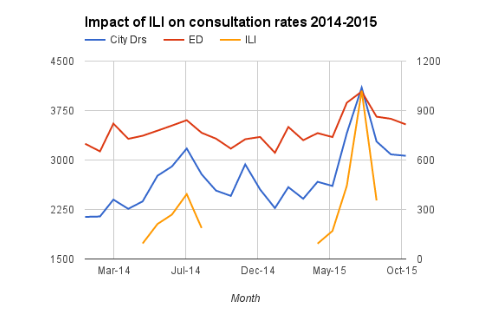
\includegraphics[scale=0.50]{ILI.png}
\caption{The short term impact of Influenza-like-illness on utilization of the Emergency department}
\label{Impact of Influenza-like-illness}
\end{figure}

The utilisation of General Practice by 5-14 shows some effect from this , but otherwise there is no significant or sustained change in service utilization (see figure 11).\\

\begin{figure}[htp]
\centering
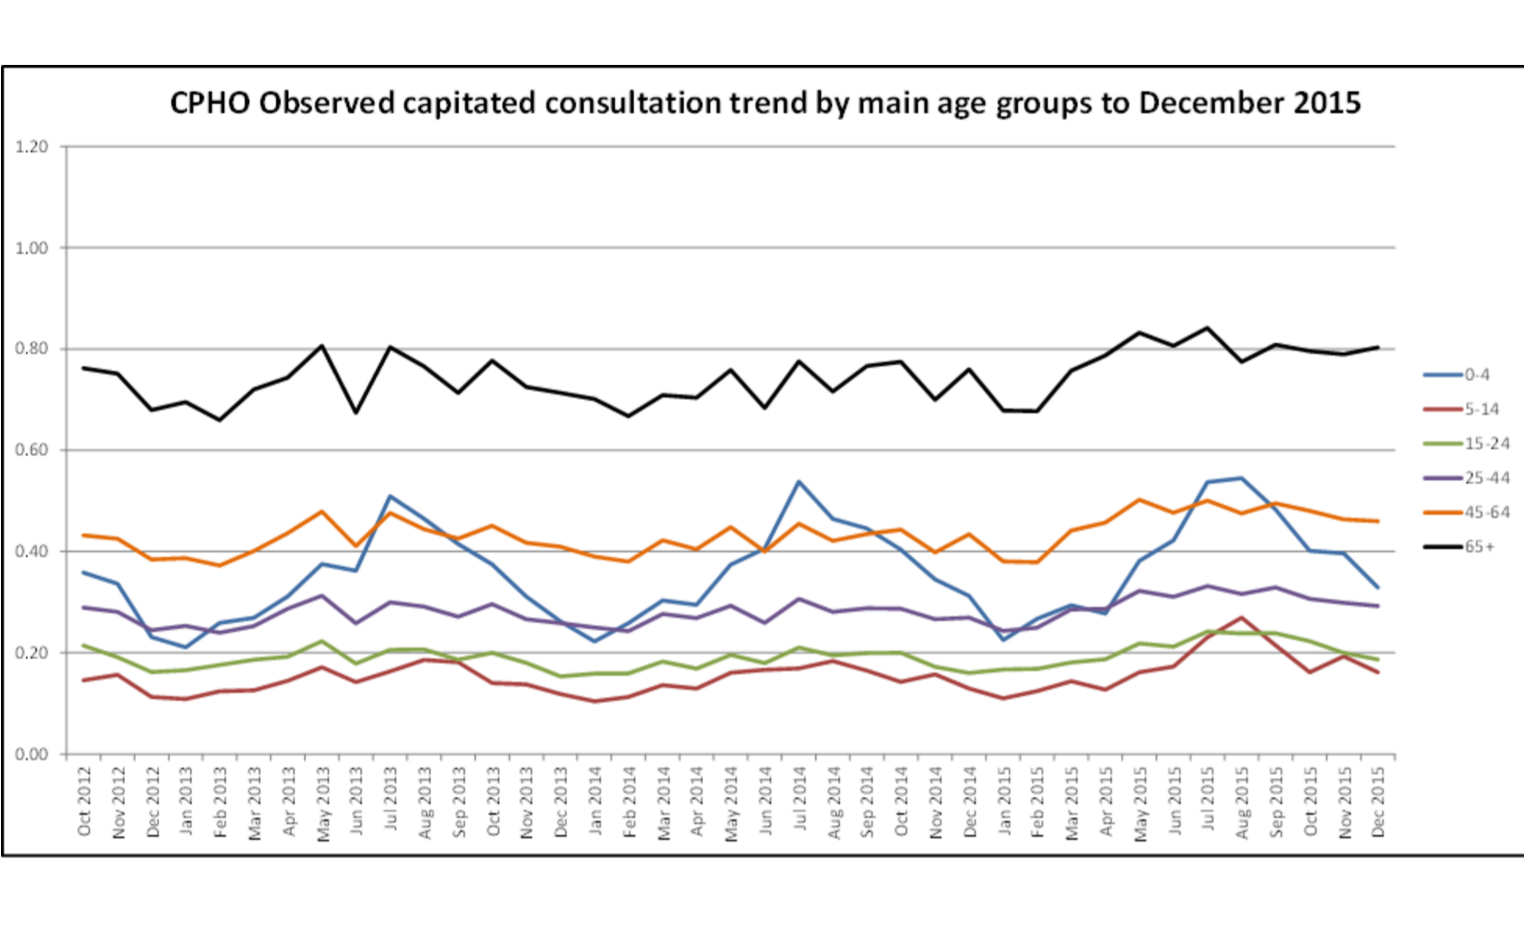
\includegraphics[scale=0.30]{U13one.png}
\caption{Stratified rates of GP consultations for Central PHO practices}
\label{Age stratified General Practice consultations}
\end{figure}

\subsection{Impacts within ED}
In contract the Emergency Department showed an immediate and sustained effect (see figure 12).

\begin{figure}[htp]
\centering
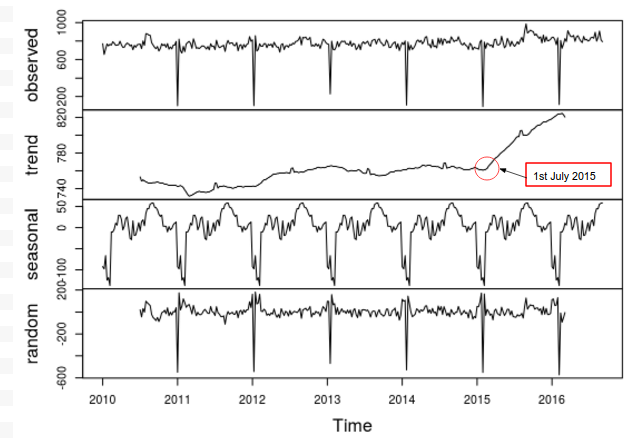
\includegraphics[scale=0.60]{TS_ED.png}
\caption{Time series analysis splitting from all Emergency Department presentations, the changing trends for utilisation from the underlying seasonal patterns.}
\label{Time series analysis of Emergency Department presentations}
\end{figure}

\begin{figure}[htp]
\centering
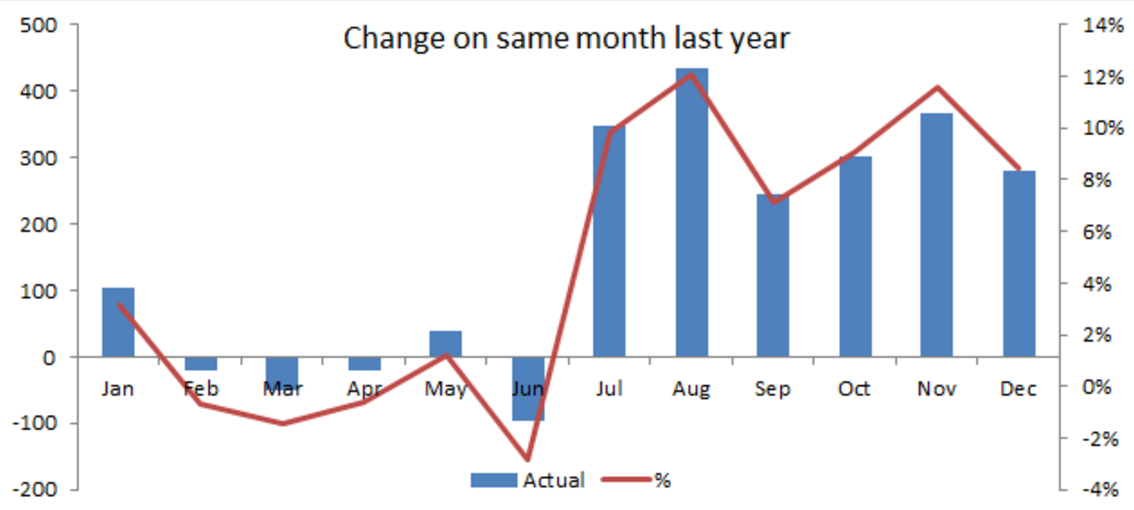
\includegraphics[scale=0.35]{ED.png}
\caption{Comparing 2015 with 2014 showing the relative increase}
\label{Relative changes in ED utilization}
\end{figure}

This change in utilisation patterns is even more marked for those who have used the department for two or three times within the same year.

\begin{figure}[htp]
\centering
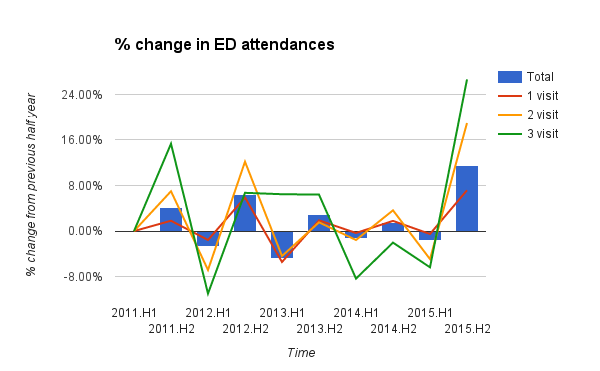
\includegraphics[scale=0.70]{Fchange.png}
\caption{Changes in ED utilisation in H2 2015, especially for rates of second and third time utilisation within the quarter}
\label{Changes in ED utilisation}
\end{figure}

The availability of primary care may be a driving factor, where availability is widely described as the ability to access urgent care either at the health home / GP team or via one of the Urgent care facilities. The presentations at ED from the four towns and their associated rural areas was plotted using both EWMA and time series plots. \\ 
\\
\\
\begin{tabular}{|l|l|}
\hline 
	Locality & Trend\\
\hline
	Palmerston North & Overall rise since 1.July.2015\\
\hline
	Horowhenua & Initial rise since 1.July.2015 but this has now stabilised\\
\hline
	Tararua & Overall rise since 1.July.2015\\
\hline
	Manawtu (Feilding) & Rise since 2012\\
\hline
\end{tabular}
\\
\\
To further investigate the impact of domicile on ED presentation following the introduction of the free 6-13 year old funding, the rate of presentation by suburb was plotted by suburb. This showed a mixed effect. There was a rise in utilisation by those suburbs who were wealthy and those with proximity to the hospital. Suburbs with high NZDep scores had a mixed result, with some increasing their Emergency Department utilisation, others decreasing.
\pagebreak

\emph{Palmerston North Suburbs}

\begin{tabular}{|l|l|}
\hline
	Suburb & Trend since 1.July.2015\\
\hline
	Kelvin Grove & Rise\\
\hline
	Milson & Rise\\
\hline
	Roslyn & Rise\\
\hline
	Papaeoia & Rise\\
\hline
	Palmerston North Central & Decrease\\
\hline
	Hokowhitu East & No change\\
\hline
	Hokowhitu Lagoon & Rise\\
\hline
	Hokowhitu West & No change\\
\hline
	Awapuni North & Rise\\
\hline
	Awapuni West & No change\\
\hline
	Awapuni South & No change\\
\hline
	Westbrook & No change\\
\hline
	Highbury & Decrease\\
\hline
	Cloverlea & Rise\\
\hline
\end{tabular}
\\
\\

\emph{Ethnicity}

To consider the impact of ethnicity, the same analysis was completed. Again a mixed pattern of results was revealed for ED utilisation.

\begin{tabular}{|l|l|}
\hline
	Ethnicity & Trend since 1.July.2015\\
\hline
	Maori & Rise\\
\hline
	NZ European & Rise\\
\hline
	Chinese & Decrease\\
\hline
	Indian & Rise\\
\hline
\end{tabular}
\\

What was not expected was the impact of different utilisation by age groups. The rise in utilisation was greatest in the over 12 year old age groups (see figure 17).\\

\begin{figure}[htp]
\centering
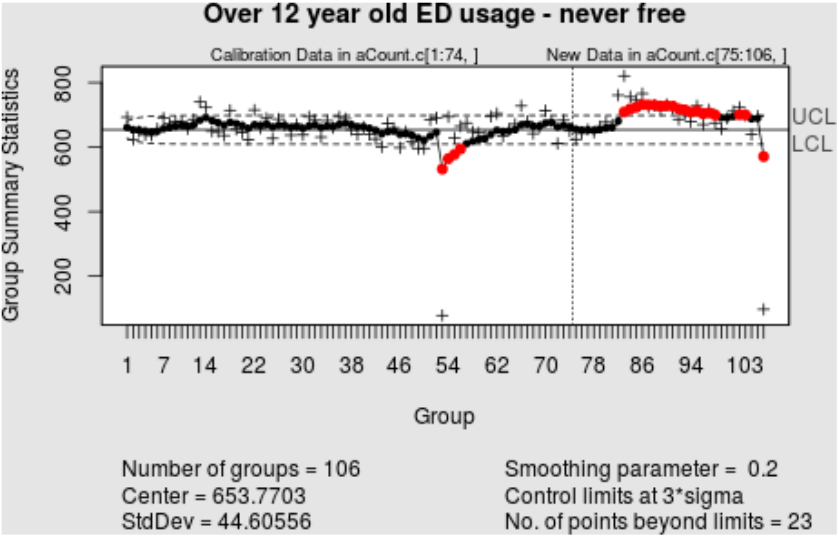
\includegraphics[scale=0.50]{Over12.png}
\caption{EWMA plot showing ED utilization by those uneffected by funding changes has risen out of control limits}
\label{Rise in ED utilisation by over 12 year olds}
\end{figure}

These changes in utilisation has persisted ever since as the new normal (see figure 18).\\

\begin{figure}[htp]
\centering
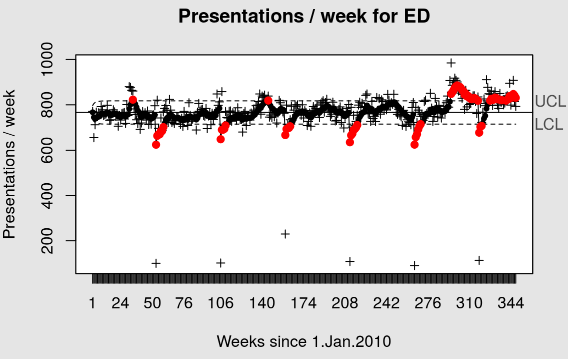
\includegraphics[scale=0.70]{EWMA_ED_pesentations.png}
\caption{EWMA chart of weekly ED presentations since 2010, with weeks put of control limits being displayed in red.}
\label{EWMA statistical process chart of ED presentations}
\end{figure}

and the projections for the future show growth continuing through until 2017, so creating a capacity crisis within the physical Emergency Department.\\

\begin{figure}[htp]
\centering
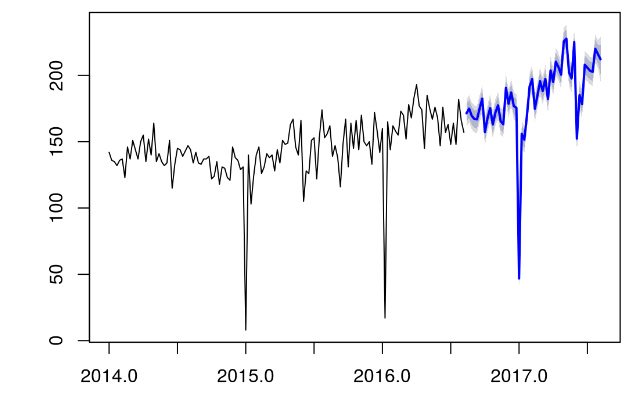
\includegraphics[scale=0.70]{HW_projections.png}
\caption{Projection for ED utilisation using a Holt-Winter's methodology.}
\label{Projections for ED utilisation through to 2017}
\end{figure}

\subsection{Impacts within the Hospital}
Increased demand for hospital based clinical care was a significant contributor to the poor fiscal result for MidCentral DHB.\\

\begin{figure}[htp]
\centering
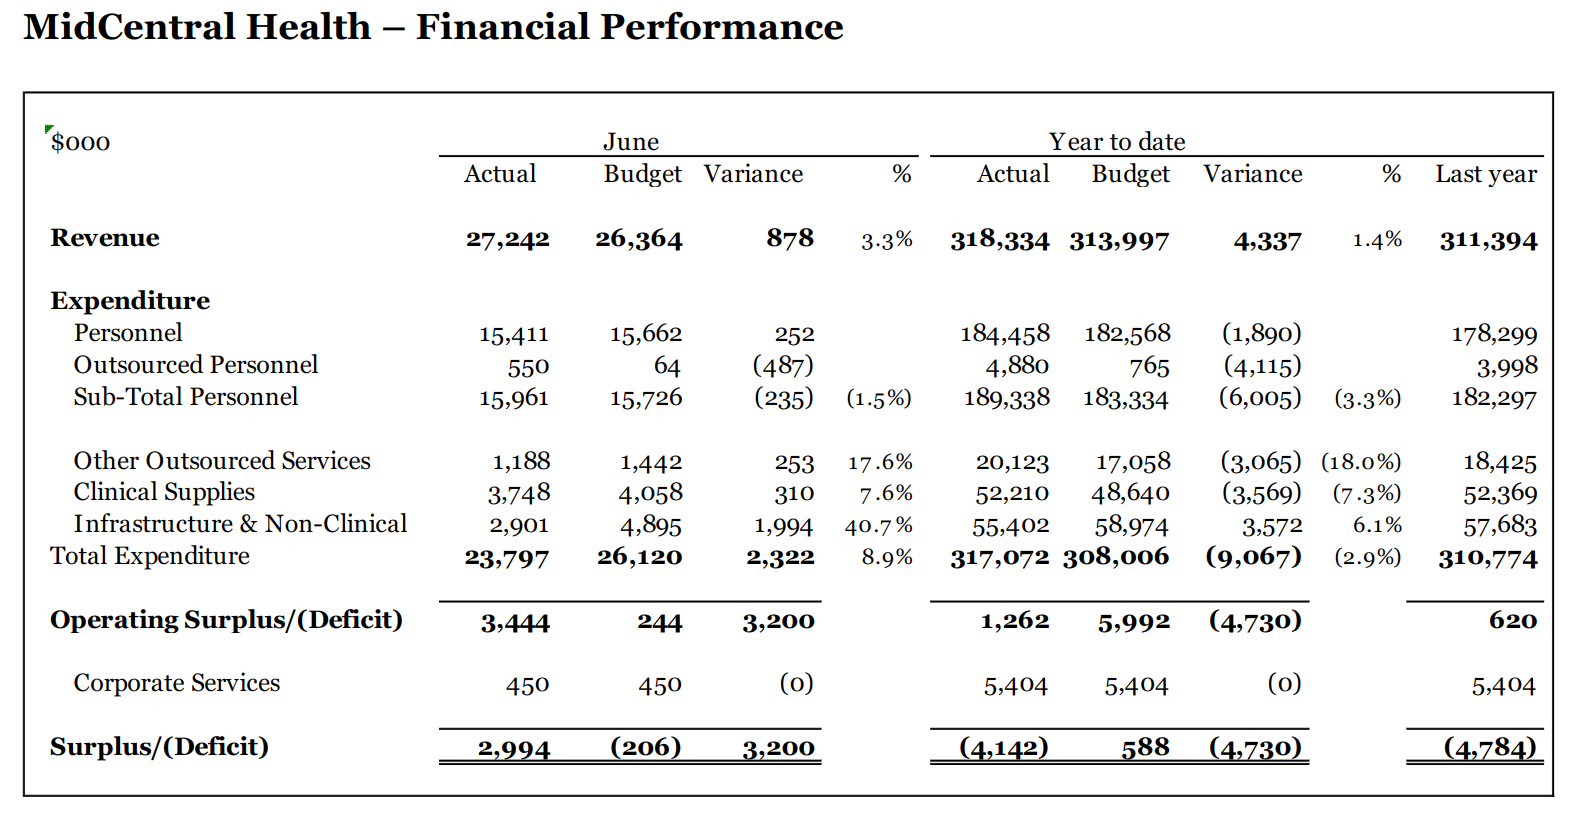
\includegraphics[scale=0.30]{MCHbalance.png}
\caption{Financial result of MidCentral Health or Palmerston North Hospital, showing a significant deficit against budget }
\label{Financial result for MidCentral Health - Palmerston North Hospital}
\end{figure}

\begin{figure}[htp]
\centering
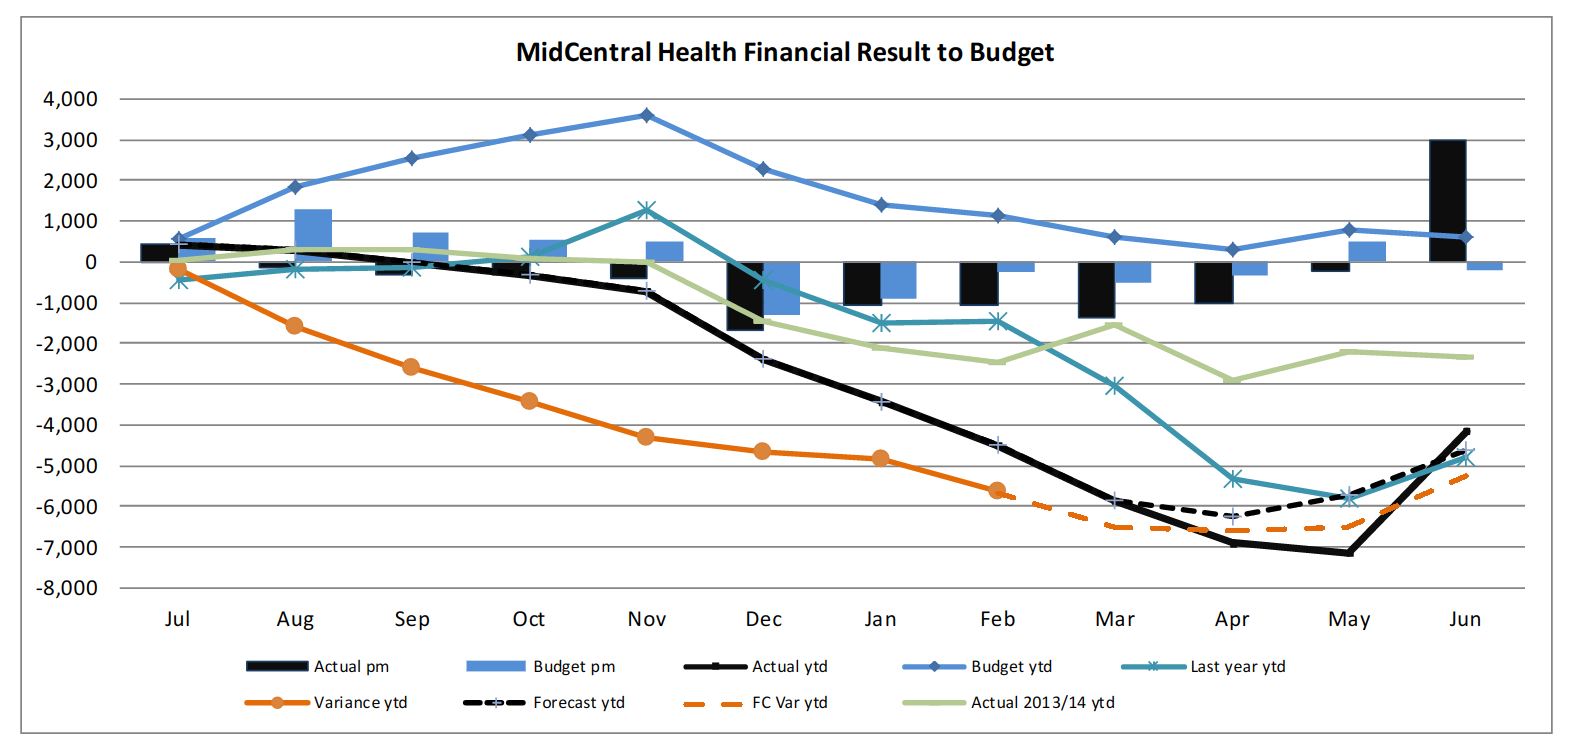
\includegraphics[scale=0.30]{MCHgraph.png}
\caption{Graphical representation of the financial performance of MidCentral Health - Palmerston North Hospital}
\label{}
\end{figure}

\pagebreak

\section{Discussion}
\citet{kerr1995folly} classic work on "the folly of rewarding A while hoping for B" springs to mind. Clearly the ability of the ability of the health sector to predict the impacts of health reforms locally is minimal. Certainly focusing on outputs not outcomes has not lead to the anticipated changes.\\

With hindsight the reforms undertaken within the Primary Health Care Strategy were more idealistic than anticipated. General Practitioners remained steeped in the "fee for service" as a business model. Capitation instead of transforming primary care into a multidisciplinary team driving preventative care, actually became a barrier to entry for new participants. Only being paid for retrospectively for enrolled patients, meant without an independent income, new practitioners had to become assistants to established practice or remain within hospital practice. Neither reality lead to a growth in equity through improved access to primary care or the growth of an internal market for the delivery of primary care through increasing the number of providers.Indeed both equity of access and the number of providers has decreased.\\

\citet{howell2005restructuring} has been proved to be correct. The size of the business units (the small 2-3 practitioner surgeries) was indeed too small to manage the risks inherent within a capitation model\citep{howell2005restructuring}. Her argument that a formal insurance model involving a larger group of patients is required to provide the risk management associated with an ageing population and shifts in utilisation patterns, is not proven by this study, but seems reasonable. \\

Her prediction was that fees would again become the primary economic driver for the financial stability of practices, has been proven to be true\citep{howell2005restructuring}. Driven by the ageing  population, there would an associated projected rise in the number of patients with chronic illnesses and multiple comorbidities that has lead to an increased  average utilisation rate, until the capacity of General Practice has been exceeded. \\

For \citet{howell2005restructuring} the size of the new IFHC that are opening is more realistic for the insurance based model to enable the achievement of the health reforms envisaged in the primary health care strategy to be achieved. Her assumption that the new IFHC will be truly integrated is not currently valid in many of the new IFHC. Many, currently, are collocated not integrated practices.\\

The various newly formed and just opening IFHC are at the start of their organisational evolution. Initially, while only collocated, they will be very vulnerable to economic forces until they develop an appropriate business model. Currently, the most common business model is that of the very large scale cohabitation of the founding practices in very large and expensive new premises. A model that dramatically increases costs without increasing income, will cause a sharp loss of shareholder value. A state that usually prompts model change. Until that change occurs then many IFHC will remain economically vulnerable. Without a change in the model of care to achieve financial sustainability, they will not be able to deliver the volume of care required to meet patient need. \\

That there is considerable unmet need especially for acute and urgent care is one interpretation of the changes in ED utilisation since 1.July.2015. The improvement of the funding for children aged under 13 years, has raised expectations as to the access to care and possibly the cost of care. \\

General Practice is saturated and patients can not gain the desired access. Instead ED through improved compliance with the six hour Ministry of health target, has become substantially (time) cheaper and is available. Hence the rise in utilisation. \\

The risks from this shift in utilisation patterns is perilous for the DHB. ED is not an infinite resource and there is physical constraints to the building, even if extra emergency department staff can be found. Unless a new building and extra staff is found, then the DHB will default on the compliance with the six hour target. If the DHB does build a new building, it will default on its financial targets and the DHB is currently on performance watch by the Ministry and keen to find a solution \footnote{http://www.stuff.co.nz/manawatu-standard/news/72250866/MidCentral-DHB-on-performance-watch-after-poor-financial-result}. \\

Care in the Emergency Department is not cheap care. Currently the cost is approximately three times the cost of urgent accident related care in an Urgent Care Clinic or about five times the cost of equivalent acute conditions being treated in General Practice. This is before the costs of any unnecessary admissions are considered. Where costs include harm to the patients.\\

These issues can only be solved through a joint approach to health service planning and implementation. Key to this shift in thinking has to be the needs of the patient, not the provider as it is currently.\\

Shifts in the model of care and delivery systems across the district are not going to happen instantly. The recommendations of this report are the first steps to achieving this shift.

\pagebreak

\bibliography{report.bib}
\end{document}

